% Based on code by Stefan Kottwitz
\documentclass[border = 10pt]{standalone}
\usepackage{tikz}
\usetikzlibrary{arrows, shapes.gates.logic.US, calc}
\usetikzlibrary{circuits.ee.IEC}
\begin{document}

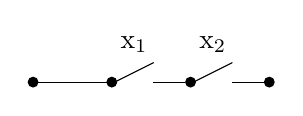
\begin{tikzpicture}
[circuit ee IEC]
\foreach \i in {1,...,4}{
	\node [contact] (contact \i) at (\i, 0) {};
}
\draw (contact 1) to (contact 2);
\draw (contact 2) to [make contact = {near start, info = x$_1$}]
 (contact 3);
\draw (contact 3) to [make contact = {near start, info = x$_2$}]
 (contact 4);
\end{tikzpicture}
\end{document}
